\documentclass[12pt]{article}

% Language setting
% Replace `english' with e.g. `spanish' to change the document language
\usepackage[english]{babel}

% Set page size and margins
% Replace `letterpaper' with `a4paper' for UK/EU standard size
\usepackage[a4paper,top=2cm,bottom=2cm,left=3cm,right=3cm,marginparwidth=1.75cm]{geometry}

% Useful packages
\usepackage{amsmath}
\usepackage{amssymb}
\usepackage{graphicx}
\usepackage{mathtools}
\usepackage{enumitem}
\usepackage[colorlinks=true, allcolors=blue]{hyperref}

%macros
\newcommand{\defeq}[2]{\stackrel{\mathclap{\normalfont\mbox{#1}}}{#2}}
\def\D{\displaystyle}
\def\att{                    % mark at the margin
        \marginpar[ \hspace*{\fill} \raisebox{-0.2em}{\rule{2mm}{1.2em}} ]
        {\raisebox{-0.2em}{\rule{2mm}{1.2em}} }
        }
\def\at#1{[*** \att #1 ***]}  % text needing attention
\def\spc{\hspace*{0.5cm}}

\title{SGD Ex}
%\author{Beryl Aribowo}

\begin{document}
\maketitle
%$asd \myeq 2$
%\at{need to rewrite this subsec with more details - the BO eq}

%%%%%%%%%%%%%%%%%%%%%%%%%%%%%%%%%%%%%%%%%%%%%%%%%%%%
\hrule
\vspace{0.1cm}
\section*{[P4]}
\subsection*{E1}
Def. 17:
\begin{equation}
    D_f(x, y) + D_f(y, x) = \langle \nabla f(x) - \nabla f(y), x - y \rangle 
                            = \langle \nabla f(y) - \nabla f(x), y - x \rangle
    \label{eq:symbregdiv}
\end{equation}
$\forall x, y \in \mathbb{R}^d $:
\begin{equation}
    \begin{split}
        \mu ||x-y||^2 & \leq 2D_f(x,y), \\
        \frac{\mu}{2} ||x-y||^2 & \leq D_f(x, y), \\
        \frac{\mu}{2} ||x-y||^2 & \leq D_f(y, x), \\
        D_f(x, y) + \frac{\mu}{2} ||x-y||^2 & \leq D_f(x, y) + D_f(y, x), \\
        D_f(x, y) + \frac{\mu}{2} ||x-y||^2 & \defeq{(\refeq{eq:symbregdiv})}{\leq} \langle \nabla f(x) - \nabla f(y), x - y \rangle.
    \end{split}
    \label{eq:E1}
\end{equation}

\subsection*{E2}
\begin{equation}
    \begin{split}
        D_f(x, y) + \frac{\mu}{2} ||x-y||^2 & \leq \langle \nabla f(x) - \nabla f(y), x - y \rangle, \\
        \langle \nabla f(x) - \nabla f(y), x - y \rangle & \geq \underbrace{D_f(x, y)}_{\geq \frac{\mu}{2} ||x-y||^2} + \frac{\mu}{2} ||x-y||^2, \\
        \langle \nabla f(x) - \nabla f(y), x - y \rangle & \geq \frac{\mu}{2} ||x-y||^2 + \frac{\mu}{2} ||x-y||^2, \\
        \langle \nabla f(x) - \nabla f(y), x - y \rangle & \geq \mu ||x-y||^2.
    \end{split}
    \label{eq:E2}
\end{equation}
\vspace{0.1cm}

%%%%%%%%%%%%%%%%%%%%%%%%%%%%%%%%%%%%%%%%%%%%%%%%%%%%
% \hrule
% \vspace{0.1cm}
% \section*{P5}
% \subsection*{E4}
% \vspace{0.1cm}

%%%%%%%%%%%%%%%%%%%%%%%%%%%%%%%%%%%%%%%%%%%%%%%%%%%%
\hrule
\vspace{0.1cm}
\section*{[P6]}
\subsection*{E17}
\subsubsection*{(Equation 34):}
\begin{equation}
    \begin{split}
        \langle a, b \rangle &\leq \frac{||a||^2}{2t} + \frac{t||b||^2}{2}, \\
        \langle a, b \rangle &\leq \frac{\langle a, a \rangle}{2t} + \frac{t \langle b, b \rangle}{2}, \\
        2t \langle a, b \rangle &\leq \langle a, a \rangle + t^2 \langle b, b \rangle, \\
        0 &\leq \langle a, a \rangle + \langle tb, tb \rangle - \langle a, tb \rangle - \langle tb, a \rangle, \\
        0 &\leq ||a - tb||^2. 
    \end{split}
\end{equation}
\subsubsection*{(Equation 35):}
\begin{equation}
    \begin{split}
        ||a+b||^2 \leq 2||a||^2 + 2||b||^2, \\
        \langle a, a\rangle + \langle b, b\rangle + 2 \langle a, b\rangle & \leq 2\langle a, a\rangle + 2\langle b, b\rangle, \\
        0 &\leq \langle a, a\rangle + \langle b, b\rangle -  2 \langle a, b\rangle, \\
        0 &\leq ||a-b||^2.
    \end{split}    
\end{equation}
\subsubsection*{(Equation 36):}
\begin{equation}
    \begin{split}
        \frac{1}{2}||a||^2 - ||b||^2 &\leq ||a+b||^2,\\
        \frac{1}{2} \langle a, a\rangle - \langle a, a\rangle &\leq \langle a, a\rangle + \langle b, b\rangle + 2 \langle a, b\rangle, \\
        \langle a, a\rangle - 2 \langle b, b\rangle &\leq 2 \langle a, a\rangle + 2 \langle b, b\rangle + 4 \langle a, b\rangle, \\
        0 &\leq \langle a, a\rangle + \langle 2b, 2b\rangle + \langle a, 2b\rangle + \langle 2b, a\rangle, \\
        0 &\leq ||a+2b||^2.
    \end{split}
\end{equation}

\subsection*{E19}
%\hyperlink{https://www.probabilitycourse.com/chapter6/6_2_2_markov_chebyshev_inequalities.php}{}
For random vector $X \in \mathbb{R}^d$:
\begin{equation}
    \textbf{\text{Var}}[X] := \textbf{E}\left[ ||X - \textbf{E}[X]||^2\right].
    \label{eq:variance}
\end{equation}
Markov's inequality:
\begin{equation}
    \text{Prob}(X \geq t) \leq \frac{\textbf{E}[X]}{t}.
    \label{eq:markovineq}
\end{equation}
Proof of Chebyshev's inequality using Markov's inequality:
\begin{equation*}
    \text{Prob}(||X - \textbf{E}[X]||^2 \geq t^2) \leq \frac{\textbf{E}\left[ ||X - \textbf{E}[X]||^2\right]}{t^2}.
\end{equation*}
Since
\begin{equation}
    \text{Prob}(||X - \textbf{E}[X]||^2 \geq t^2) = \text{Prob}(||X - \textbf{E}[X]|| \geq t),
\end{equation}
then
\begin{equation}
    \text{Prob}(||X - \textbf{E}[X]|| \geq t) \leq \frac{\textbf{Var}[X]}{t^2}.
\end{equation}
\vspace{0.1cm}

%%%%%%%%%%%%%%%%%%%%%%%%%%%%%%%%%%%%%%%%%%%%%%%%%%%%
\hrule
\vspace{0.1cm}
\section*{[P7]}
\subsection*{E24}
If
\begin{equation*}
    f = \frac{1}{n} \sum^n_{i=1}f_i,
\end{equation*}
then
\begin{equation*}
    \begin{split}
        D_f(x, y) &= \frac{1}{n} \sum^n_{i=1} f_i(x) - 
                \frac{1}{n} \sum^n_{i=1} f_i(y) - 
                \frac{1}{n} \sum^n_{i=1} \langle \nabla f_i(y), x-y \rangle, \\
        D_f(x, y) &= \frac{1}{n} \sum^n_{i=1} (f_i(x) - f_i(y) - \langle \nabla f_i(y), x-y \rangle), \\
        D_f(x, y) &= \frac{1}{n} \sum^n_{i=1} D_{f_i}(x, y).
    \end{split}
\end{equation*}
\subsection*{E26}
If $\sigma^2_\star = 0$, then
\begin{equation*}
    \begin{split}
        \sigma^2_\star &= \left(\frac{1}{n^2} \sum_{i=1}^n \frac{||\nabla f_i(x^\star)||^2}{p_i}\right) - ||\nabla f(x^\star)||^2 = 0 \\
        &= \left(\frac{1}{n^2} \sum_{i=1}^n \frac{||np_i \nabla f(x^\star)||^2}{p_i}\right) - ||\nabla f(x^\star)||^2 = 0\\
        &= p_i \sum_{i=1}^n (|| \nabla f(x^\star) ||^2) - ||\nabla f(x^\star)||^2 = 0\\
        &= np_i || \nabla f(x^\star) ||^2 - ||\nabla f(x^\star)||^2 = 0, \\
        \sigma^2_\star = 0 &\implies np_i \nabla f(x^\star) = \nabla f(x^\star).
    \end{split}
\end{equation*}
\vspace{0.1cm}

%%%%%%%%%%%%%%%%%%%%%%%%%%%%%%%%%%%%%%%%%%%%%%%%%%%%
\hrule
\vspace{0.1cm}
\section*{[P8]}
\subsection*{E33}
Let
\begin{equation*}
    \chi_i = 
    \begin{cases}
        1 \quad i \in S\\
        0 \quad i \notin S
    \end{cases}
    .
\end{equation*}
Since
\begin{equation*}
    p_i = \frac{1}{n},
\end{equation*}
and
\begin{equation*}
    |S| = \tau,
\end{equation*}
then 
\begin{equation*}
    \textbf{E}[\chi_i] = \text{Prob}(i \in S) = \sum^n_{i=1} p_i \chi_i = \frac{1}{n} \sum^n_{i=1} \chi_i = \frac{\tau}{n}.
\end{equation*}

\subsection*{E35}
For any vectors, $b_1, ..., b_n \in \mathbb{R}^d$:
\begin{equation*}
    \begin{split}
        \left\|\sum^n_{i=1} b_i \right\|^2 - \sum^n_{i=1}  \left\| b_i \right\|^2 &= \underbrace{\sum^n_{i=1} \langle b_i, b_i\rangle + \sum_{i \neq j} \langle b_i, b_j \rangle}_{\left\|\sum^n_{i=1} b_i \right\|^2} - \sum^n_{i=1} \langle b_i, b_i\rangle, \\
        \left\|\sum^n_{i=1} b_i \right\|^2 - \sum^n_{i=1}  \left\| b_i \right\|^2 &= \sum_{i \neq j} \langle b_i, b_j \rangle.
    \end{split}
\end{equation*}

%%%%%%%%%%%%%%%%%%%%%%%%%%%%%%%%%%%%%%%%%%%%%%%%%%%%
\hrule
\vspace{0.1cm}
\section*{[P9]}
\subsection*{E37}
Assumptions of $\mathcal{C}:\mathbb{R}^d \rightarrow \mathbb{R}^d$ :
\begin{enumerate}
    \item $\mathbf{E}[\mathcal{C}(x)] = x, \quad \forall x \in \mathbb{R}^d$
    \item $\mathbf{E}\left[||\mathcal{C}(x) - x||^2\right] \leq \omega ||x ||^2 + \delta, \quad \forall x \in \mathbb{R}^d, \quad \exists \omega, \delta \geq 0$
\end{enumerate}
Proof of convergence for CGD with $n=1$: \\
Since $\mathcal{C} \in \mathbb{B}^d(\omega)$,
\vspace{0.2cm}
\begin{equation}
    \mathbf{E}\left[ ||g(x)||^2 \right] = \mathbf{E}\left[||\mathcal{C}(\nabla f(x)) ||^2\right] \leq (\omega + 1) || \nabla f(x)||^2.
    \label{eq:expectation_gx}
\end{equation}
In case of $\nabla f(y) = 0$,
\begin{equation*}
    \begin{split}
        G(x,y) &:= \mathbf{E}\left[ ||g(x) - \nabla f(y)||^2 \right] \\
            &= \mathbf{E}\left[ ||g(x)||^2 \right] \\
            &\defeq{(\ref{eq:expectation_gx})}{\leq} (\omega + 1)||\nabla f(x) - \nabla f(y)||^2, \\
            &\leq 2(\omega + 1)LD_f(x,y).
    \end{split}
\end{equation*}
In case of $\nabla f(y) \neq 0$,
\begin{equation*}
    \begin{split}
        G(x,y) &:= \mathbf{E}\left[ ||g(x) - \nabla f(y)||^2 \right] \\
                &= \mathbf{E}\left[ ||g(x) - \nabla f(x)||^2 \right] + || \nabla f(x) - \nabla f(y)||^2 \\
                &= \mathbf{E}\left[ ||\mathcal{C}(\nabla f(x)) - \nabla f(x)||^2 \right] + ||\nabla f(x) - \nabla f(y)||^2 \\
                &\leq \omega ||\nabla f(x)||^2 + \delta + || \nabla f(x) - \nabla f(y)||^2 \\
                &= \omega ||\nabla f(x) - \nabla f(y) + \nabla f(y)||^2 + || \nabla f(x) - \nabla f(y)||^2 + \delta \\
                &\leq 2\omega||\nabla f(x) - \nabla f(y)||^2 + 2\omega|| \nabla f(y) ||^2 + || \nabla f(x) - \nabla f(y)||^2 + \delta \\
                &= (2\omega+1)||\nabla f(x) - \nabla f(y)||^2 + 2\omega|| \nabla f(y) ||^2 + \delta \\
                &\leq 2\underbrace{(2\omega+1)L}_{A}D_f(x,y) + \underbrace{2\omega||\nabla f(y)||^2 + \delta}_{C}.
    \end{split}
\end{equation*}
If $0 < \gamma < \frac{1}{A}$, then
\begin{equation*}
    \mathbf{E}\left[ ||x^k - x^*||^2 \right] \leq (1-\gamma \mu)^k ||x^0 - x^* || + \frac{2\gamma\omega|| \nabla f(x^*)||^2 + \gamma\delta}{\mu}.
\end{equation*}

\subsection*{E39}
Lemma 51: \\
if $\mathcal{C}(x) = x, \forall x$ (no master compression) and $\omega_i = \omega,\forall i$, then
\begin{equation*}
    \begin{split}
        G(x,y) \leq 2 \underbrace{\left(L + 2L_{\text{max}}\frac{\omega}{n}\right)}_{A}D_f(x,y) + \underbrace{2\frac{\omega}{n}\sigma^2(y)}_{C(y)},
    \end{split}
\end{equation*}
where
\begin{equation*}
    \sigma^2(y) := \frac{1}{n}\sum_{i=1}^n ||\nabla f_i(y)||^2.
\end{equation*}
If $\sigma^2(y) = 0$, then
\begin{equation*}
    G(x,y) \leq 2 \underbrace{\left(L + L_{\text{max}}\frac{\omega}{n}\right)}_{A}D_f(x,y).
\end{equation*}
\textbf{Proof}: \\
If $\nabla f(y) \neq 0$, then
\begin{equation}
    \begin{split}
        G(x,y) &:= \mathbf{E}\left[ ||g(x) - \nabla f(y)||^2 \right] \\
                &= \mathbf{E}\left[ ||g(x) - \nabla f(x)||^2 \right] + ||\nabla f(x) - \nabla f(y)||^2 \\
                &\leq \mathbf{E}\left[ ||g(x) - \nabla f(x)||^2 \right] + 2LD_f(x,y),
    \end{split}
\end{equation}
and
\begin{equation}
    \begin{split}
        g(x)   = \mathcal{C}(\hat{g}(x)) = \hat{g}(x) = \frac{1}{n}\sum_{i=1}^n g_i(x).
    \end{split}
    \label{eq:p9g}
\end{equation}
where
\begin{equation*}
    g_i(x) = \mathcal{C}_i(\nabla f_i (x)).
\end{equation*}
Estimate
\begin{equation*}
    \begin{split}
        \mathbf{E}\left[ ||g(x) - \nabla f(x)||^2 \right] &\defeq{(\ref{eq:p9g})}{=} \mathbf{E}\left[ ||\mathcal{C}(\hat{g}(x)) - \nabla f(x)||^2 \right] \\
                &= \mathbf{E}\left[ ||\hat{g}(x) - \nabla f(x)||^2 \right] \\
                &= \mathbf{E}\left[ \left\| \frac{1}{n} \sum_{i=1}^n \underbrace{(g_i(x) - \nabla f_i(x))}_{a_i}\right\|^2\right] \\
                &= \frac{1}{n^2} \mathbf{E}\left[\sum_{i=1}^n ||a_i||^2 + \sum_{i\neq j}\langle a_i, a_j \rangle \right] \\
                &= \frac{1}{n^2} \sum_{i=1}^n \mathbf{E}\left[||a_i||^2\right] + \sum_{i\neq j} \mathbf{E}\left[\langle a_i, a_j \rangle \right] \\
                &= \frac{1}{n^2} \sum_{i=1}^n \mathbf{E}\left[||a_i||^2\right] + \sum_{i\neq j} \langle \underbrace{\mathbf{E}\left[a_i\right]}_{0}, \underbrace{\mathbf{E}\left[a_j\right]}_{0} \rangle \\
                &\leq \frac{1}{n^2} \sum_{i=1}^n \omega_i || \nabla f_i (x)||^2 \\
                &= \frac{\omega}{n^2} \sum_{i=1}^n || \nabla f_i (x)||^2.
    \end{split}
\end{equation*}
Next, bound
\begin{equation*}
    \begin{split}
        || \nabla f_i(x)||^2 &= || \nabla f_i(x) - \nabla f_i(y) + \nabla f_i(y)||^2 \\
                            &\leq 2|| \nabla f_i(x) - \nabla f_i(y)||^2 + 2 || \nabla f_i(y)||^2 \\
                            &\leq 4L_iD_{f_i}(x,y) + 2 ||\nabla f_i(y)||^2.
    \end{split}
\end{equation*}
Combine everything:
\begin{equation}
    \begin{split}
        G(x, y) &\leq \mathbf{E}\left[ ||g(x) - \nabla f(x)||^2 \right] + 2LD_f(x,y) \\
                &\leq \frac{\omega}{n^2} \sum_{i=1}^n || \nabla f_i (x)||^2 + 2LD_f(x,y) \\
                &\leq \frac{\omega}{n^2} \sum_{i=1}^n \left( 4L_iD_{f_i}(x,y) + 2 ||\nabla f_i(y)||^2 \right) + 2LD_f(x,y) \\
                &= 2 \frac{\omega}{n} \left(2 \sum_{i=1}^n \frac{1}{n} L_iD_{f_i}(x,y) + \frac{1}{n} \sum_{i=1}^n ||\nabla f_i(y)||^2 \right)+ 2LD_f(x,y) \\
                &\leq  2 \frac{\omega}{n}\left({2}L_{\text{max}}D_f(x,y) + \sigma^2(y) \right)+ 2LD_f(x,y) \\
                &= 2(L + 2L_{\text{max}})D_f(x,y) + 2 \frac{\omega}{n} \sigma^2(y).
    \end{split}
    \label{eq:gxy_deltanotzero}
\end{equation}
Else, if $\nabla f(y) = 0$, then
\begin{equation}
    \begin{split}
        G(x, y) &= \mathbf{E}\left[ ||\hat{g}(x)||^2 \right] \\
                &= \mathbf{E}\left[ ||\hat{g}(x) - \mathbf{E}\left[ \hat{g}(x) \right]||^2 \right] + ||\mathbf{E}\left[ \hat{g}(x) \right]||^2 \\
                &= \mathbf{E}\left[ ||\hat{g}(x) - \nabla f(x)||^2 \right] + || \nabla f(x)||^2\\
                &\leq \left(\frac{\omega}{n^2} \sum_{i=1}^n ||\nabla f_i(x)||^2 \right) + || \nabla f(x) - \nabla f(y) + \nabla f(y)||^2 \\
                &\leq \left(\frac{\omega}{n^2} \sum_{i=1}^n ||\nabla f_i(x)||^2 \right) + 2|| \nabla f(x) - \nabla f(y)||^2 + 2|| \underbrace{\nabla f(y)}_{0}||^2\\
                &\leq \left(\frac{\omega}{n^2} \sum_{i=1}^n ||\nabla f_i(x)||^2 \right) + 2LD_f(x,y)  \\
                &\leq ... \text{ same as (\ref{eq:gxy_deltanotzero}), from the third line} \\
                &= 2(L + 2L_{\text{max}})D_f(x,y) + 2 \frac{\omega}{n} \sigma^2(y).
    \end{split}
\end{equation}
% \begin{figure}
%     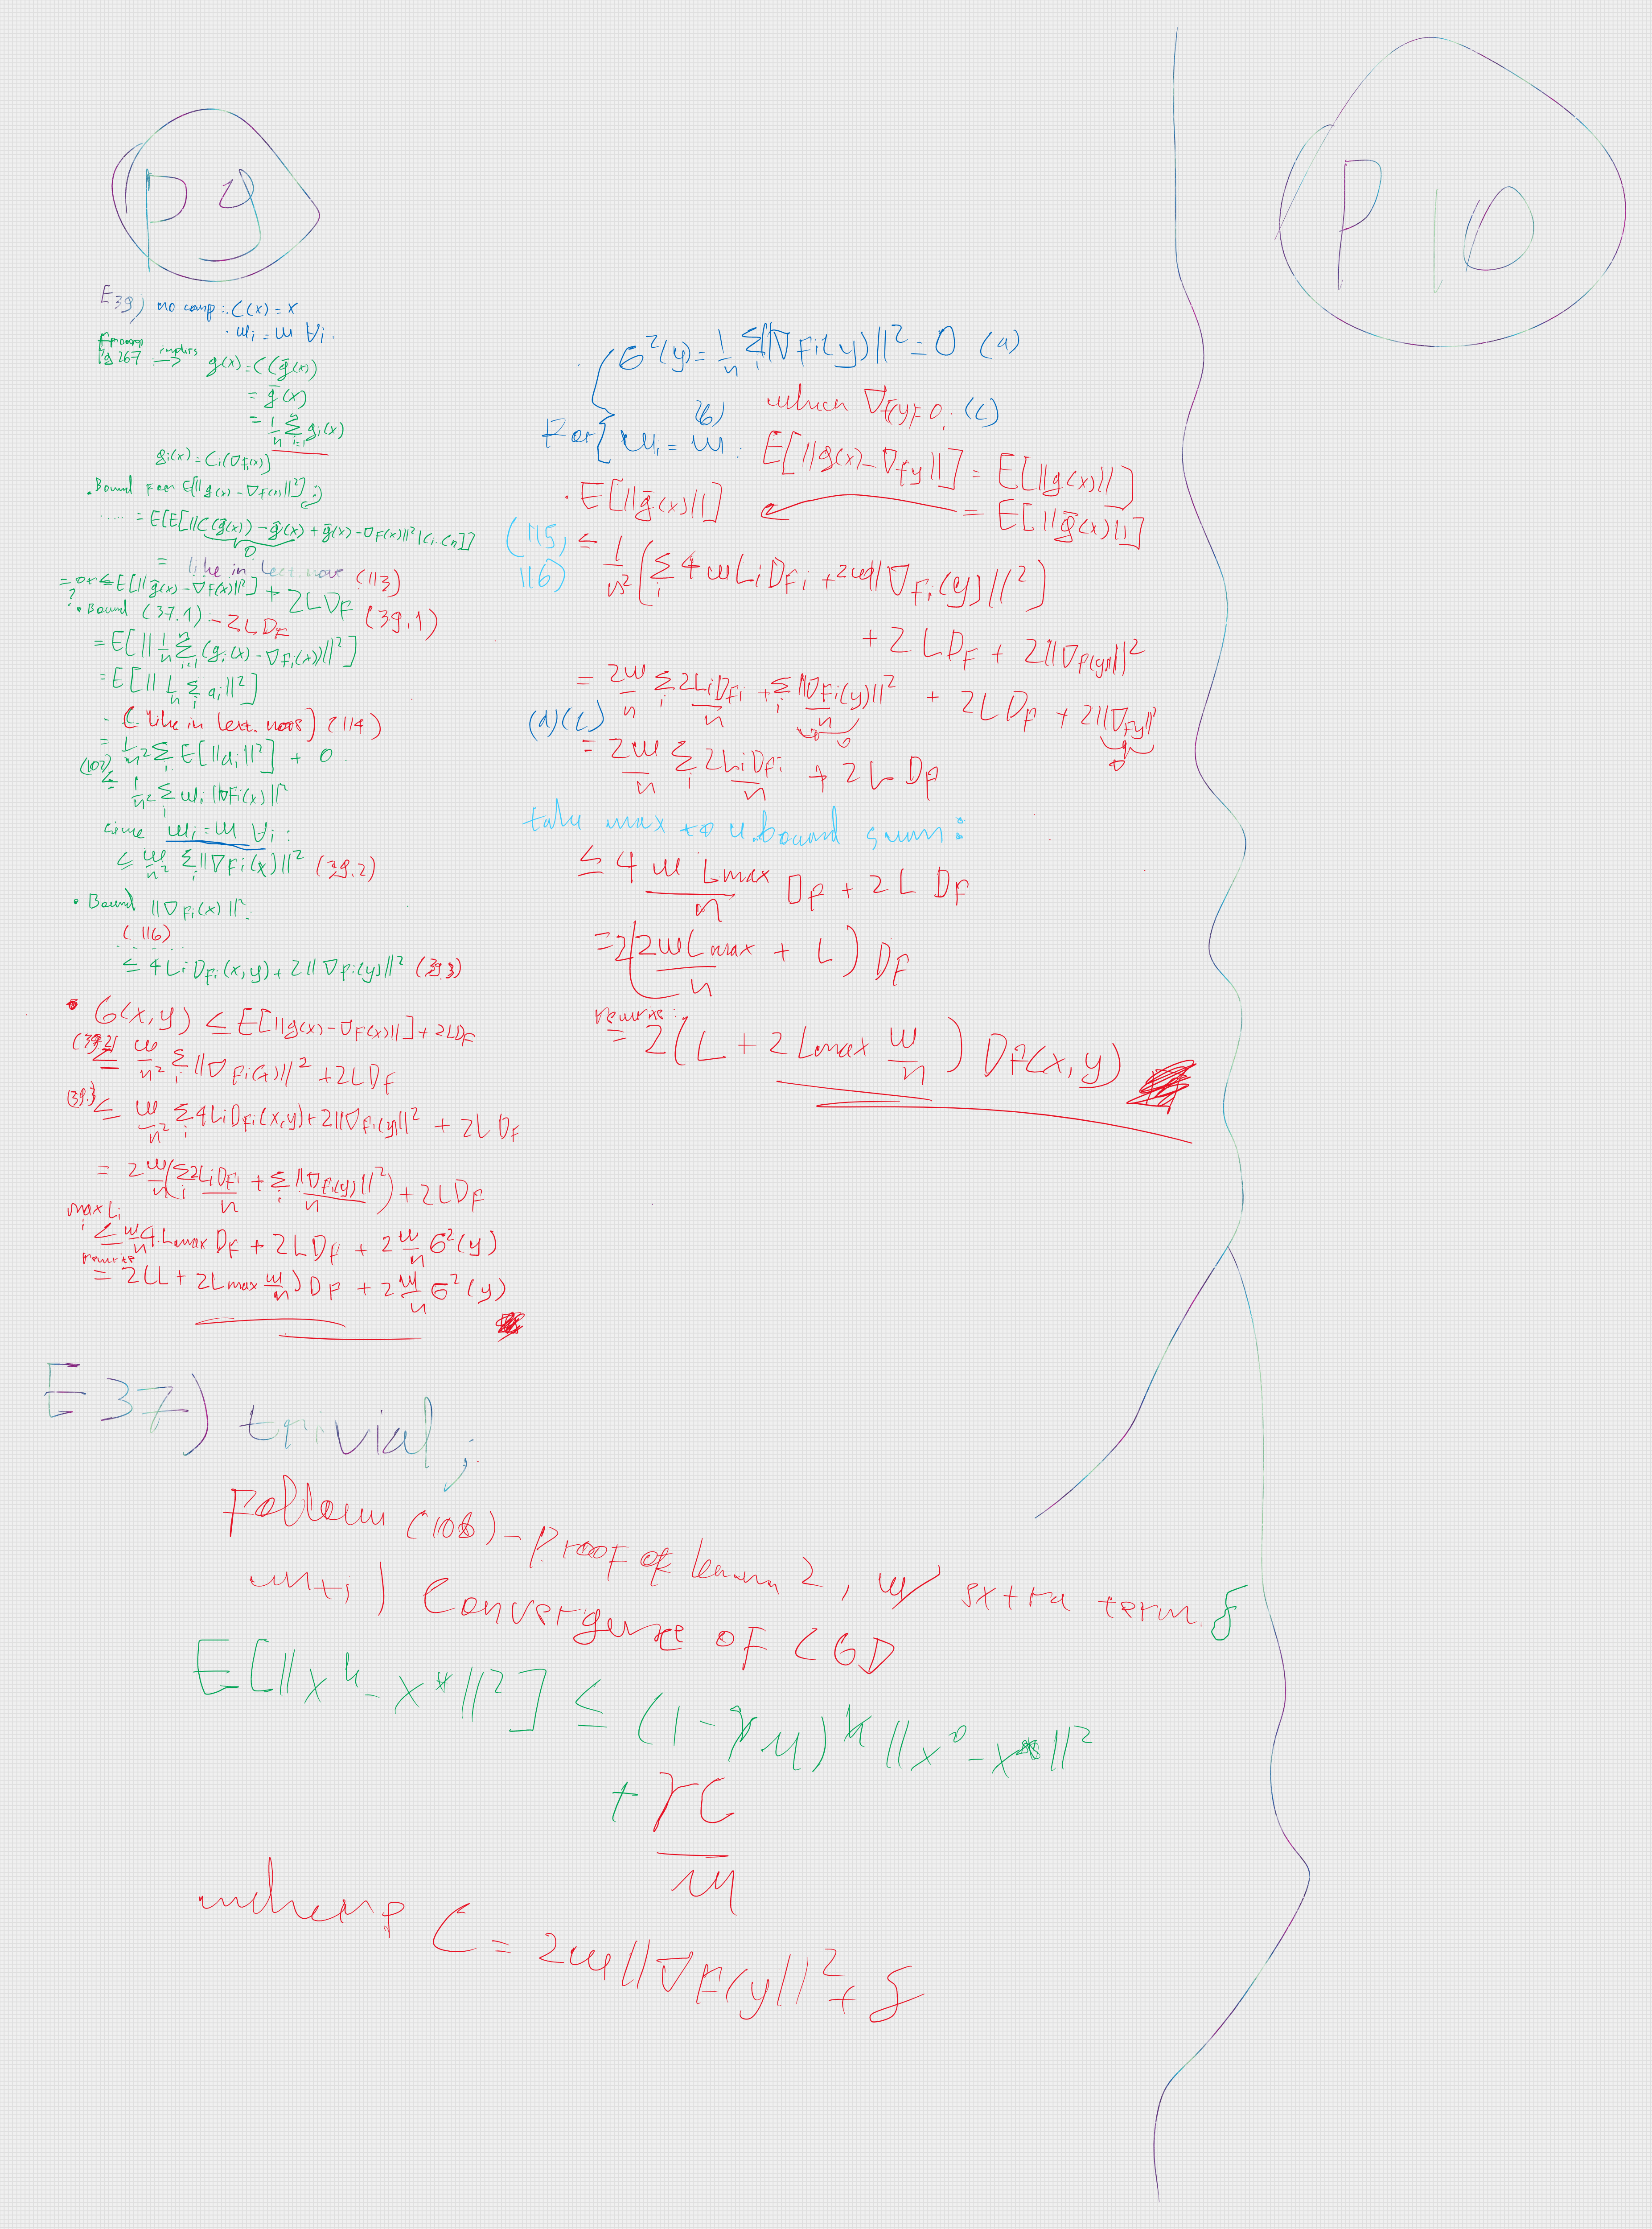
\includegraphics[width=\textwidth,height=\textheight,keepaspectratio]{img/P9.png}
% \end{figure}

%%%%%%%%%%%%%%%%%%%%%%%%%%%%%%%%%%%%%%%%%%%%%%%%%%%%
\hrule
\vspace{0.1cm}
\section*{[P10]}
\subsection*{E41}
Let
\begin{equation*}
    p_i = \text{Prob}(i \in S),
\end{equation*}
where
\begin{equation*}
    S \subseteq \{1,2,...,d\},
\end{equation*}
then
\begin{equation*}
    \mathbf{E}[|S|] = \mathbf{E}\left[\sum_{i=1}^d |S_i|\right] = \sum_{i=1}^d \mathbf{E}[|S_i|] = \sum_{i=1}^d 1p_i + 0(1-p_i) = \sum_{i=1}^d p_i.
\end{equation*}

\subsection*{E42}
If $\mathbf{E}[\mathbf{C}^\top\mathbf{C}]$ is finite, then $\forall x \neq 0$:
\begin{equation*}
    \begin{split}
        x^T \mathbf{E}[\mathbf{C}^\top\mathbf{C}] x &\geq 0 \\
        \mathbf{E}[x^T \mathbf{C}^\top\mathbf{C}x ] &\geq 0 \\
        x^T \mathbf{C}^\top\mathbf{C}x &\geq 0 \\
        (\mathbf{C}x)^\top(\mathbf{C}x) &\geq 0.
    \end{split}
\end{equation*}

%\hyperlink{https://math.stackexchange.com/questions/2650892/expectation-of-positive-semidefinite-random-matrix}{}

%%%%%%%%%%%%%%%%%%%%%%%%%%%%%%%%%%%%%%%%%%%%%%%%%%%%
\hrule
\vspace{0.1cm}
\section*{[P11]}
\subsection*{E47}
Define base case:
\begin{equation*}
    \begin{split}
        C_{1,2} &:= C_1 \circ C_2 \in \mathbb{B}^d(\underbrace{(\omega_1 + 1)(\omega_2 + 1) - 1}_{\omega_{1,2}}), \\
        C_{1,3} &:= C_1 \circ C_2 \circ C_3 = C_{1,2} \circ C_{3}, \\
        \omega_{1,3} &:= (\omega_{1,2} + 1)(\omega_{3} + 1) - 1 \\
                &= ((\omega_{1} + 1)(\omega_{2} + 1) - 1 + 1)(\omega_{3} + 1) - 1 \\
                &= (\omega_{1} + 1)(\omega_{2} + 1)(\omega_{3} + 1) - 1, \\
                C_{1,n} &:= C_1 \circ C_2 \circ ... \circ C_n = C_{1,n-1} \circ C_{n}, \\
                \omega_{1,n} &:= (\omega_{1} + 1)(\omega_{2} + 1) ... (\omega_{n} + 1) - 1 = (\omega_{1,n-1}+1)(\omega_{n}+1)-1.
    \end{split}
\end{equation*}
By induction, the base case is clear. Next, if $n=k$, assume
\begin{equation*}
    \begin{split}
        C_{1,k} &:= C_1 \circ C_2 \circ ... \circ C_k = C_{1,k-1} \circ C_{k}, \\
        \omega_{1,k} &:= (\omega_{1} + 1)(\omega_{2} + 1) ... (\omega_{k} + 1) - 1 = (\omega_{1,k-1}+1)(\omega_{k}+1)-1
    \end{split}
\end{equation*}
is true. Then for $n = k+1$:
\begin{equation*}
    \begin{split}
        C_{1,k+1} &:= C_1 \circ C_2 \circ ... \circ C_k \circ C_{k+1} = C_{1,k-1} \circ C_{k} \circ C_{k+1}, \\
        \omega_{1,k+1} &:= (\omega_{1,k}+1)(\omega_{k+1}+1)-1 = (\omega_{1} + 1)(\omega_{2} + 1) ... (\omega_{k} + 1)(\omega_{k+1} + 1) - 1 \\
                        &:= ((\omega_{1,k-1}+1)(\omega_{k}+1)-1 + 1)(\omega_{k+1}+1)-1 = (\omega_{1} + 1)(\omega_{2} + 1) ... (\omega_{k} + 1)(\omega_{k+1} + 1) - 1\\
                        &:= ((\omega_{1} + 1)(\omega_{2} + 1) ... (\omega_{k} + 1))(\omega_{k+1}+1)-1 = (\omega_{1} + 1)(\omega_{2} + 1) ... (\omega_{k} + 1)(\omega_{k+1} + 1) - 1, \\
        \omega_{1,k+1} &= (\omega_{1} + 1)(\omega_{2} + 1) ... (\omega_{k} + 1)(\omega_{k+1} + 1) - 1.
    \end{split}
\end{equation*}

\subsection*{E48}
Define
\begin{equation*}
    \min \{a_i, b_i\} = 
    \begin{cases}
        a_i, \text{ if } a_i < b_i \\
        b_i, \text{ if } a_i > b_i
    \end{cases}
    .
\end{equation*}
Thus
\begin{equation*}
    \sum_i \min \{a_i, b_i\} = 
    \begin{cases}
        \sum_i a_i, \text{ if } a_i < b_i, \forall i \\
        \sum_i b_i, \text{ if } a_i > b_i, \forall i
    \end{cases}
    .
\end{equation*}
In case of inequality, define
\begin{equation*}
    \begin{split}
        I := \{i|a_i < b_i \}, \\
        J := \{i|a_i > b_i\}    .
    \end{split}
\end{equation*}
Thus
\begin{equation*}
    \begin{split}
        \sum_i \min\{a_i, b_i\} <
        \begin{cases}
            \sum_i a_i, \text{ if } |I| > |J| \\
            \sum_i b_i, \text{ if } |J| > |I|
        \end{cases}
        .
    \end{split}
\end{equation*}

%%%%%%%%%%%%%%%%%%%%%%%%%%%%%%%%%%%%%%%%%%%%%%%%%%%%
\hrule
\vspace{0.1cm}
\section*{[P12]}
\subsection*{E55}
The DCGD-SHIFT has the same exact steps in the algorithm as DCGD ($n\geq 1$ case), the difference is the gradient estimator:
\begin{equation}
    g_h(x) := \frac{1}{n} \sum_{i=1}^n g_{h_i}(x) = \frac{1}{n} \sum_{i=1}^n h_i + \mathcal{C}_i(\nabla f_i(x) - h_i).
    \label{dcgd_shift_estimator}
\end{equation}
which means the gradients on the workers are shifted and then compressed. Decompose
\begin{equation*}
    \mathbf{E}\left[||g_h(x^k) - \nabla f(x^\star) ||^2\right] = \mathbf{E}\left[||g_h(x^k) - \nabla f(x^k) ||^2\right] + ||\nabla f(x^k) - \nabla f(x^\star) ||^2.
\end{equation*}
Then, bound
\begin{equation*}
    \begin{split}
        \mathbf{E}\left[||g_h(x^k) - \nabla f(x^k) ||^2\right] &= \mathbf{E}\left[\left\|\frac{1}{n} \sum_{i=1}^n \underbrace{\mathcal{C}_i(\nabla f_i(x^k) - h_i) + h_i - \nabla f_i(x^k)}_{b_i^k}  \right\|^2\right] \\
        &= \frac{1}{n^2} \mathbf{E}\left[\sum_i ||b_i^k||^2 \sum_{i\neq j} \langle b_i^k, b_j^k\rangle\right] \\
        &= \frac{1}{n^2} \sum_{i=1}^n \mathbf{E}\left[||b_i^k||^2\right] + \frac{1}{n^2} \sum_{i \neq j} \underbrace{\langle \mathbf{E}[b_i^k], \mathbf{E}[b_j^k] \rangle}_{0} \\
        &= \frac{1}{n^2} \sum_{i=1}^n \mathbf{E}\left[\left\| \mathcal{C}_i(\nabla f_i(x^k) - h_i) + h_i - \nabla f_i(x^k) \right\|^2\right] \\
        &\leq \frac{1}{n^2} \sum_{i=1}^n \omega_i || \nabla f_i(x^k) - h_i ||^2 \\
        &= \frac{1}{n^2} \sum_{i=1}^n \omega_i || \nabla f_i(x^k) - \nabla f_i(x^\star) - (h_i - \nabla f_i(x^\star))||^2 \\
        &\leq \frac{2}{n^2} \sum_{i=1}^n \omega_i||\nabla f_i(x^k) - \nabla f_i(x^\star)||^2 + \omega_i || h_i - \nabla f_i(x^\star) ||^2 \\
        &\leq \frac{2}{n^2} \sum_{i=1}^n 2 \omega_i L_i D_{f_i}(x^k,x^\star) + \frac{2}{n^2} \sum_{i=1}^n \omega_i || h_i - \nabla f_i(x^\star) ||^2 \\
        &\leq \frac{4}{n} \max(L_i \omega_i) \frac{1}{n} \sum_{i=1}^n D_{f_i}(x^k, x^\star) + \frac{2}{n^2} \sum_{i=1}^n \omega_i || h_i - \nabla f_i(x^\star) ||^2 \\
        &\leq \frac{4}{n} \max(L_i \omega_i) D_{f_i}(x^k, x^\star) + \frac{2}{n^2} \sum_{i=1}^n \omega_i || h_i - \nabla f_i(x^\star) ||^2.
    \end{split}
\end{equation*}
Thus
\begin{equation*}
    \mathbf{E}\left[||g_h(x^k) - \nabla f(x^\star) ||^2\right] \leq 2 \underbrace{(L + \frac{2}{n}\max(\omega_i L_i))}_{A}D_f(x^k, x^\star) + \underbrace{\frac{2}{n^2}\sum_{i=1}^n \omega_i ||h_i - \nabla f_i(x^\star)||^2}_{C}.
\end{equation*}

%%%%%%%%%%%%%%%%%%%%%%%%%%%%%%%%%%%%%%%%%%%%%%%%%%%%
\hrule
\vspace{0.1cm}
\section*{[P13]}
\subsection*{E56}
Thm 94: whenever $B=0$ and $M=0$, then $\frac{B+M\tilde{B}}{M} = 0$, proof:\\
First, the stepsize $\gamma$ satisfies
\begin{equation}
    0 < \gamma < \frac{1}{\mu}.
    \label{eq:94gamma}
\end{equation}
Then the iterates $\{x^k, \sigma^k\}$ satisfy
\begin{equation}
    \mathbf{E}[d^k] \leq (1-\gamma\mu)^k d^0 + \frac{C\gamma}{\mu}.
    \label{eq:94iterate}
\end{equation}
where
\begin{equation}
    d^k := \left\| x^k - x^\star \right\|^2.
\end{equation}
From Lemma 95, it is clear
\begin{equation*}
    \begin{split}
        \mathbf{E}[d^{k+1}] &\leq (1-\gamma\mu)\mathbf{E}[d^k] + C\gamma^2.
    \end{split}
\end{equation*}
By recurrence, we obtain
\begin{equation*}
    \mathbf{E}[d^{k}] \leq (1-\gamma\mu)^k d^0 + \frac{C\gamma}{\mu}.
\end{equation*}

%%%%%%%%%%%%%%%%%%%%%%%%%%%%%%%%%%%%%%%%%%%%%%%%%%%%
\hrule
\vspace{0.1cm}
\section*{[P14]}
\subsection*{E57}
In case of arbitrary $p$, the gradient estimator of L-SVRG is
\begin{equation*}
    g^k := g(x^k) - g(y^k) + \nabla f(y^k).
\end{equation*}
Hence, the unbiasedness:
\begin{equation*}
    \begin{split}
        \mathbf{E}[g^k|x^k, y^k] &= \mathbf{E}[g(x^k) - g(y^k) + \nabla f(y^k)|x^k, y^k] \\
        &= \mathbf{E}[g(x^k)|x^k, y^k] - \mathbf{E}[g(y^k)|x^k, y^k] + \mathbf{E}[\nabla f(y^k)|x^k, y^k] \\
        &= \nabla f(x^k) - \nabla f(y^k) + \nabla f(y^k)\\
        &= \nabla f(x^k).
    \end{split}
\end{equation*}

\subsection*{E58}
If
\begin{equation*}
    g(x) = \nabla f(x) + \xi,
\end{equation*}
then
\begin{equation*}
    \begin{split}
        g^k &= (\nabla f(x^k) + \xi) - (\nabla f(y^k) + \xi) + \nabla f(y^k) \\
            &= \nabla f(x^k),
    \end{split}
\end{equation*}
which is exactly GD's gradient estimator, where in this case $p$ does not have any role, since the gradient estimator does not depend on $y^k$ anymore. 
The convergence rate in this case, with stepsize $\gamma = \frac{1}{6A''}$ is
\begin{equation*}
    \mathbf{E}[d^k] \leq \left(1 - \frac{\mu}{6A''}\right)^kd^0,
\end{equation*}
where
\begin{equation*}
    d^k := \left\| x^k - x^\star \right\|^2.
\end{equation*}
Thus
\begin{equation*}
    k \geq \frac{6A''}{\mu}\log\frac{1}{\epsilon},
\end{equation*}
which is equal to GD's rate of $\mathcal{O}\left(\frac{L}{\mu}\log\frac{1}{\epsilon}\right)$.

%%%%%%%%%%%%%%%%%%%%%%%%%%%%%%%%%%%%%%%%%%%%%%%%%%%%
\hrule
\vspace{0.1cm}
\section*{[P15]}
\subsection*{E57}

\end{document}